\documentclass[a4paper]{article}
\usepackage{hyperref}
\usepackage{graphicx}
\title{Banchetto di elettronica}
\author{Mariano Mollo, Ferdinando D'Apice}
\date{2022/05/06}
\begin{document}
\maketitle{}

Queste note sul banchetto di elettronica sono state scritte dalle note per il
banchetto dei PONYS a Futuro Remoto nel 2021\footnote{
  \url{https://ponys.notion.site/Elettronica-4e432c12fe2a40dd824e0322ac21edcf} }
e dalle note prodotte per il laboratorio portato a Parla Potabile nel 2022.

\begin{figure}[ht]
  \centering
  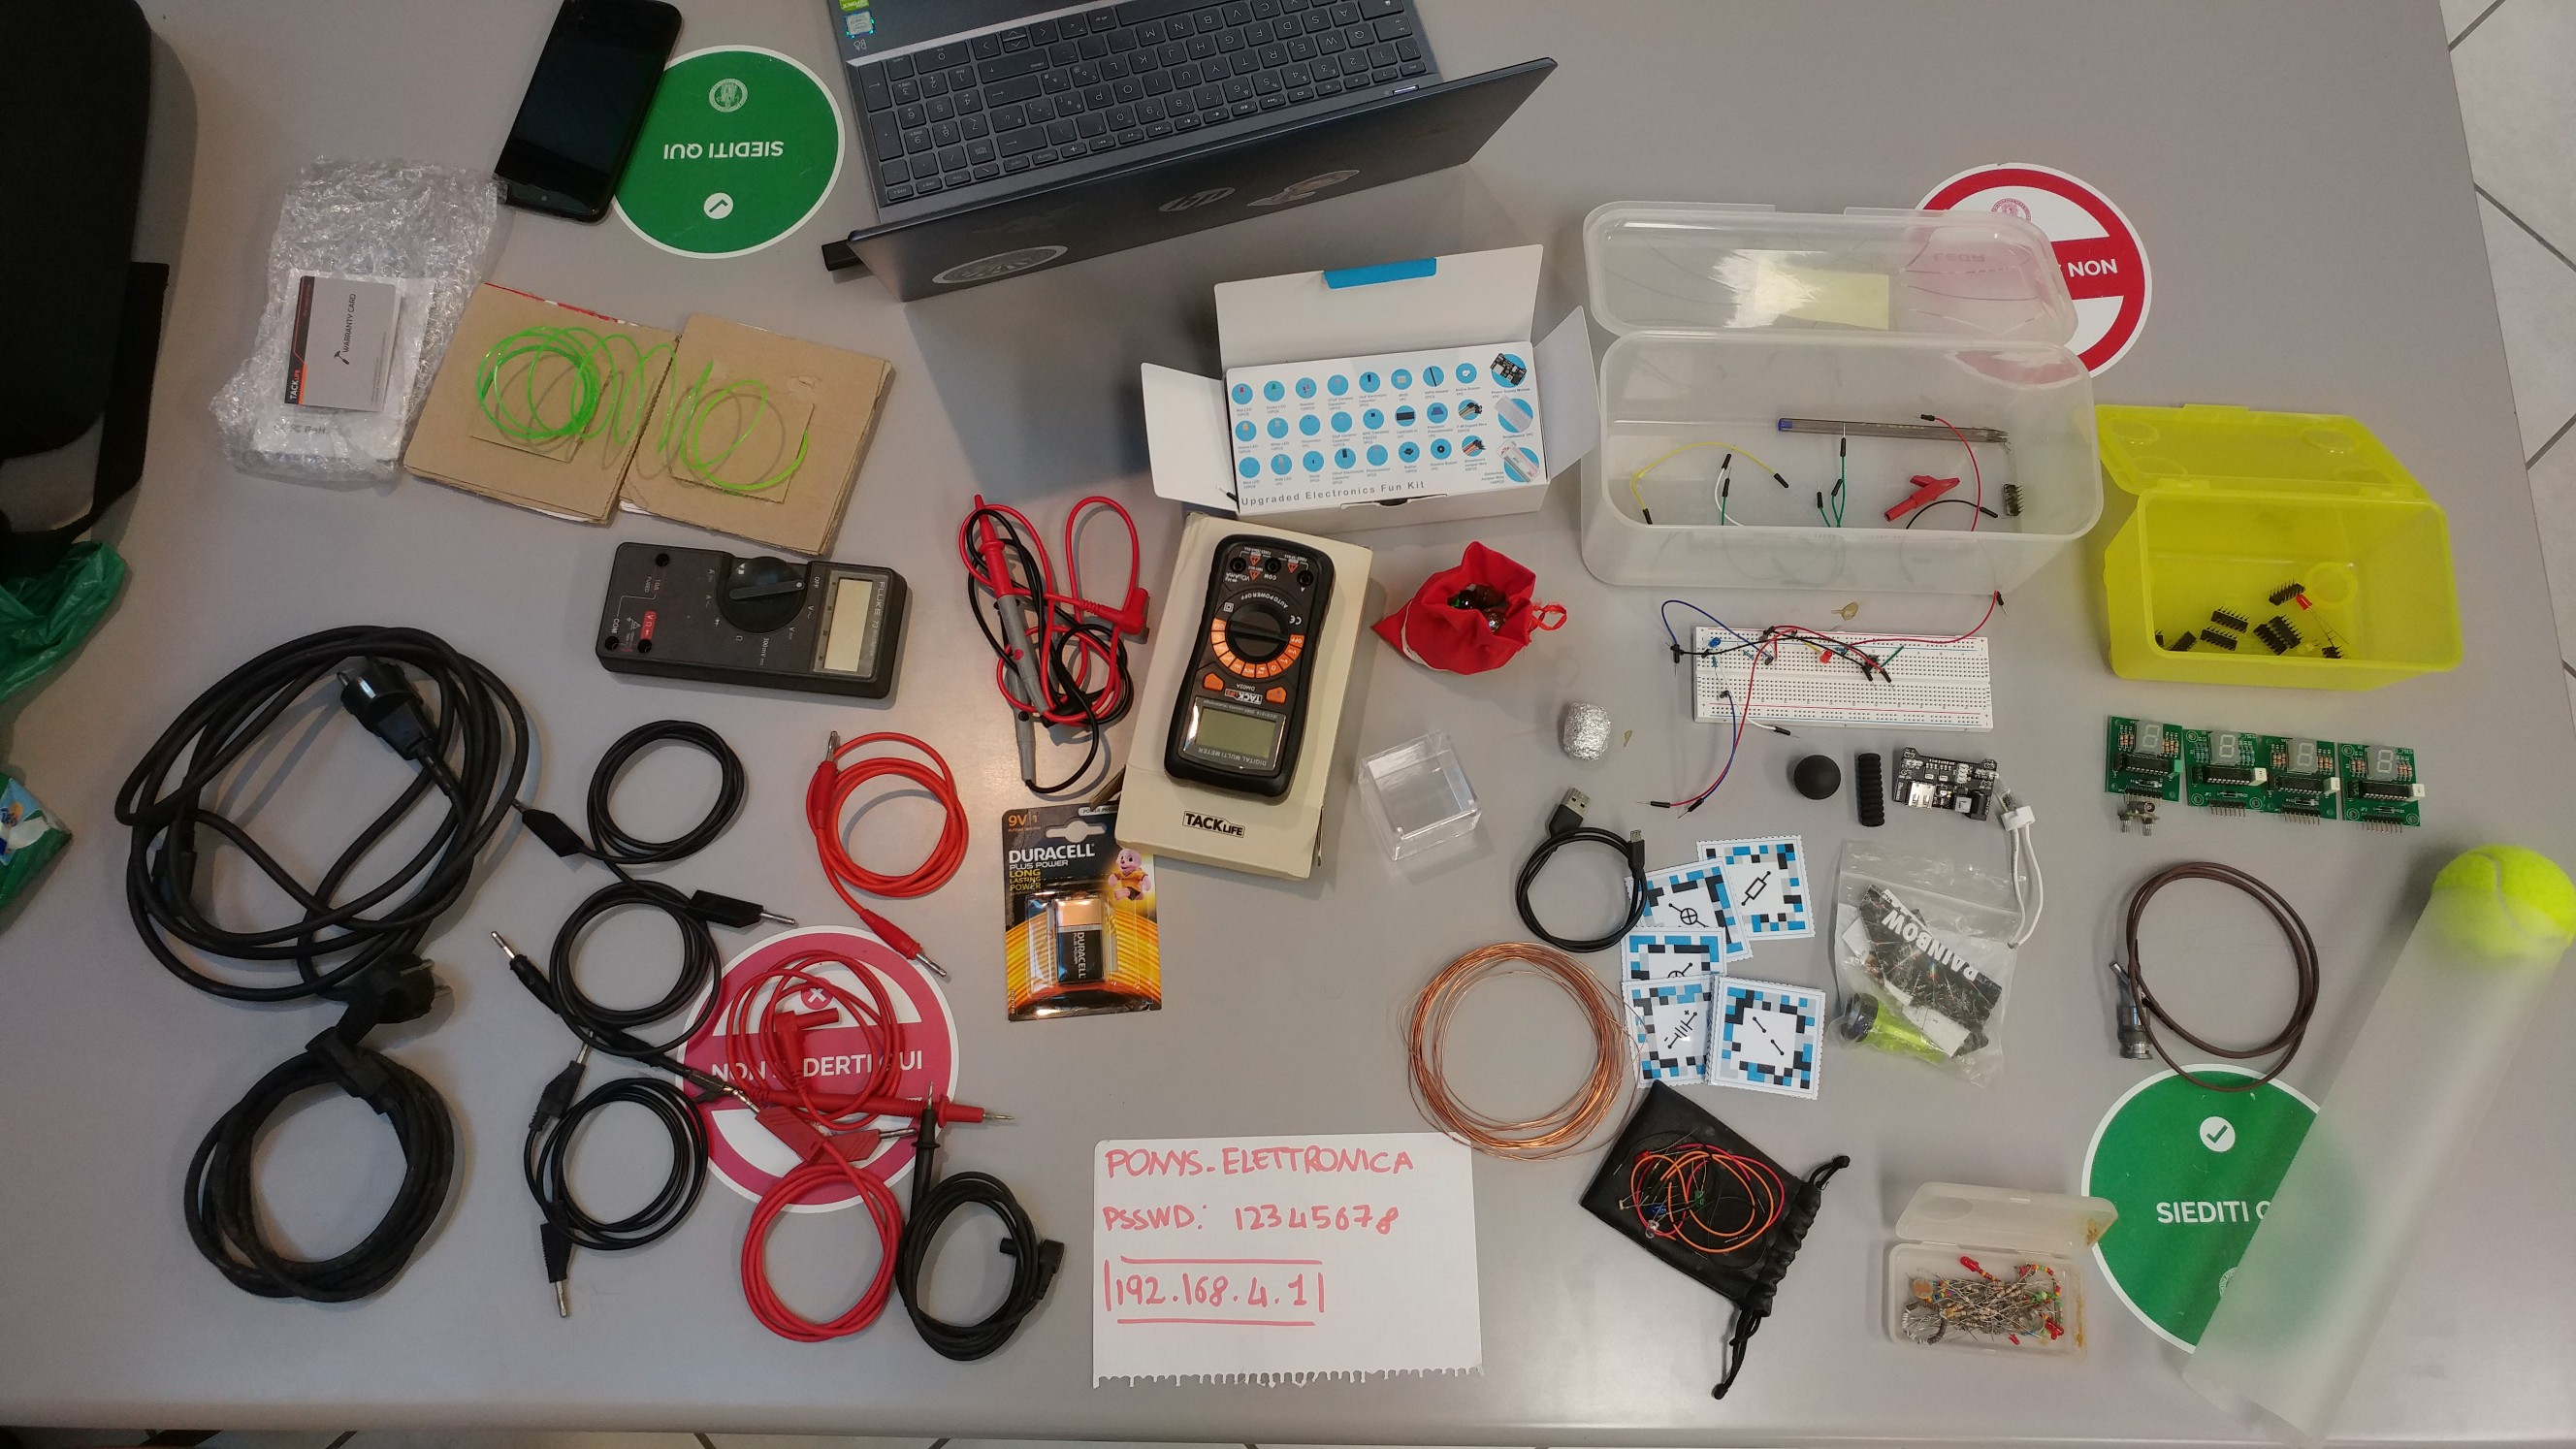
\includegraphics[angle=90, width=\linewidth]{figures/panoramica_materiale}
  \caption{\label{fig:panoramica} Panoramica del materiale}
\end{figure}

\begin{figure}[ht]
  \centering
  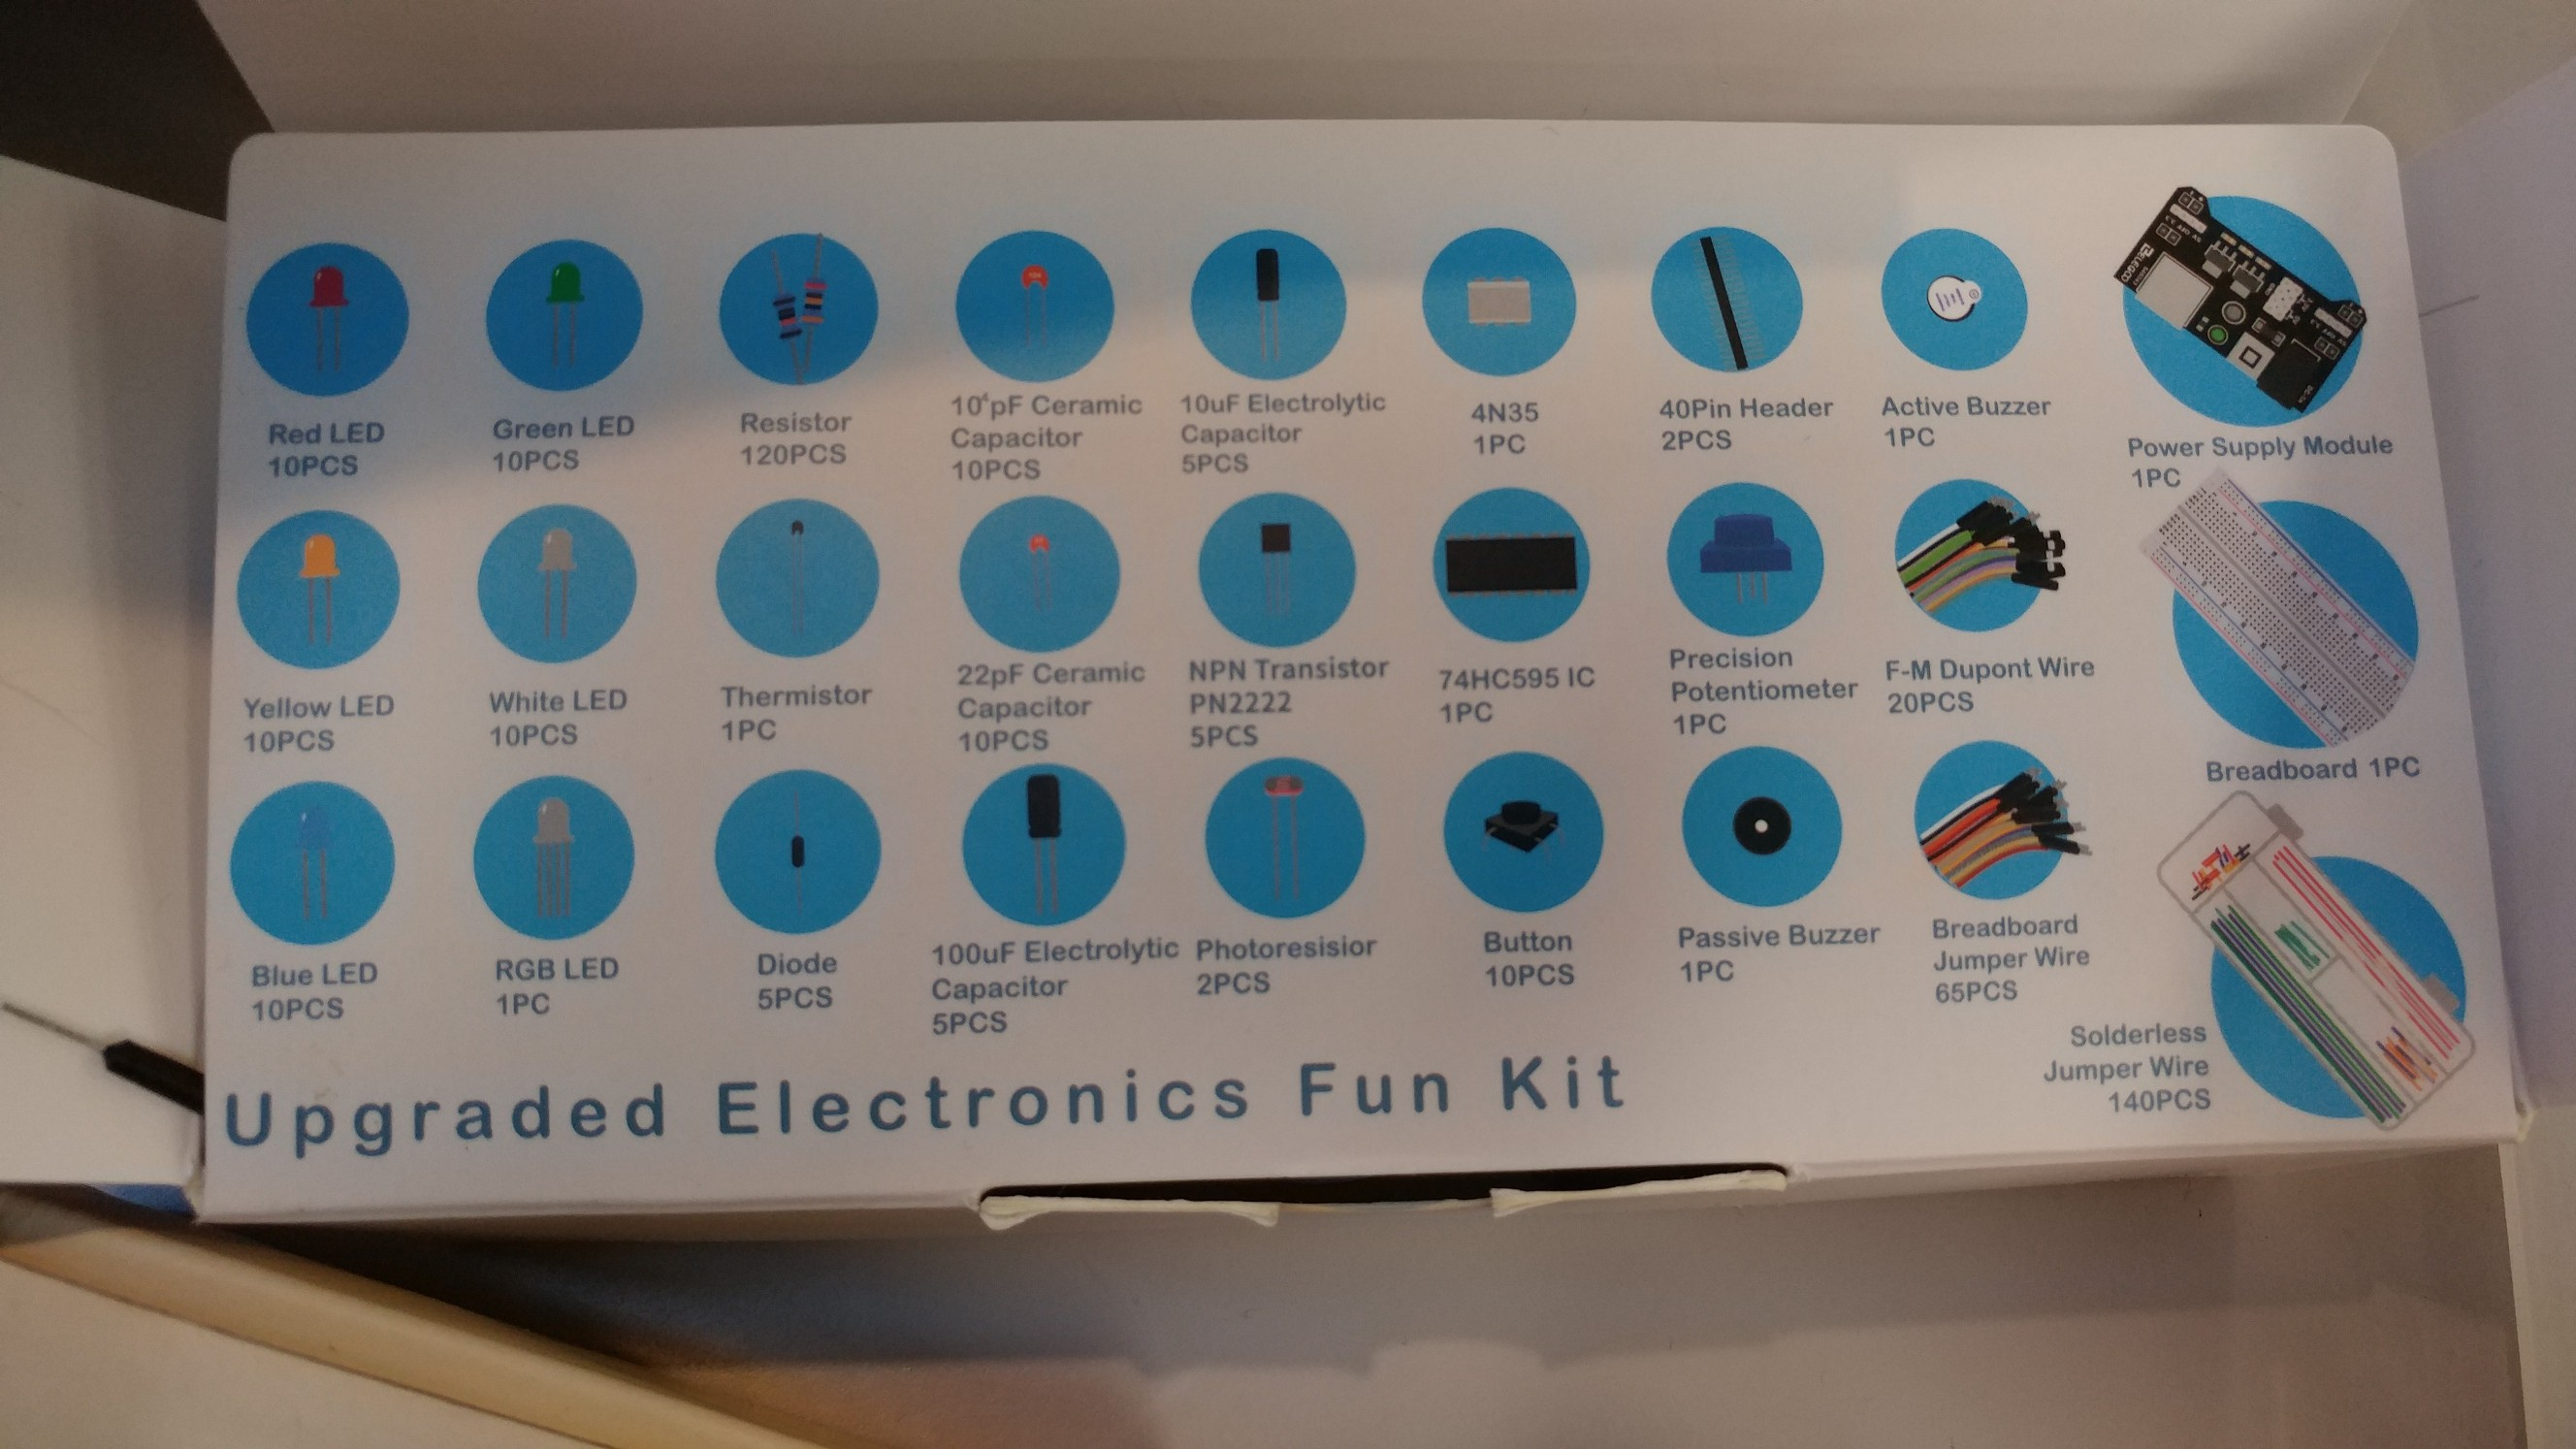
\includegraphics[width=\linewidth]{figures/kit_elettronica}
  \caption{\label{fig:kit} Kit di elettronica}
\end{figure}

\section{Spiegazione del fenomeno}%
\label{sec:fenomeno}

Si può illustrare il movimento delle cariche elettriche sotto effetto del
potenziale elettrostatico con alcune analogie dal mondo della gravitazione e
della fluidodinamica. Una pallina in interazione con il potenziale
gravitazionale si muoverà dall'alto in basso sotto effetto della gravità. Si
mostri questo usando un tubo trasparente e delle biglie che si muovono al suo
interno a seconda che si elevi una estremità o l'altra\footnote{ In realtà
  questa visualizzazione non rappresenta fedelmente ciò che accade nella realtà:
  \url{https://www.youtube.com/watch?v=oI_X2cMHNe0} }. Le biglie si muoveranno
diversamente anche a seconda del fluido che attraversano. Si immagini che una
pallina che cade nell'acqua o nel miele avrà velocità diverse. Al variare della
temperatura inoltre il miele cambierà la propria viscosità. La viscosità si
collega alla resistenza dunque di un conduttore attraversato da elettroni.

\begin{figure}[ht]
  \centering
  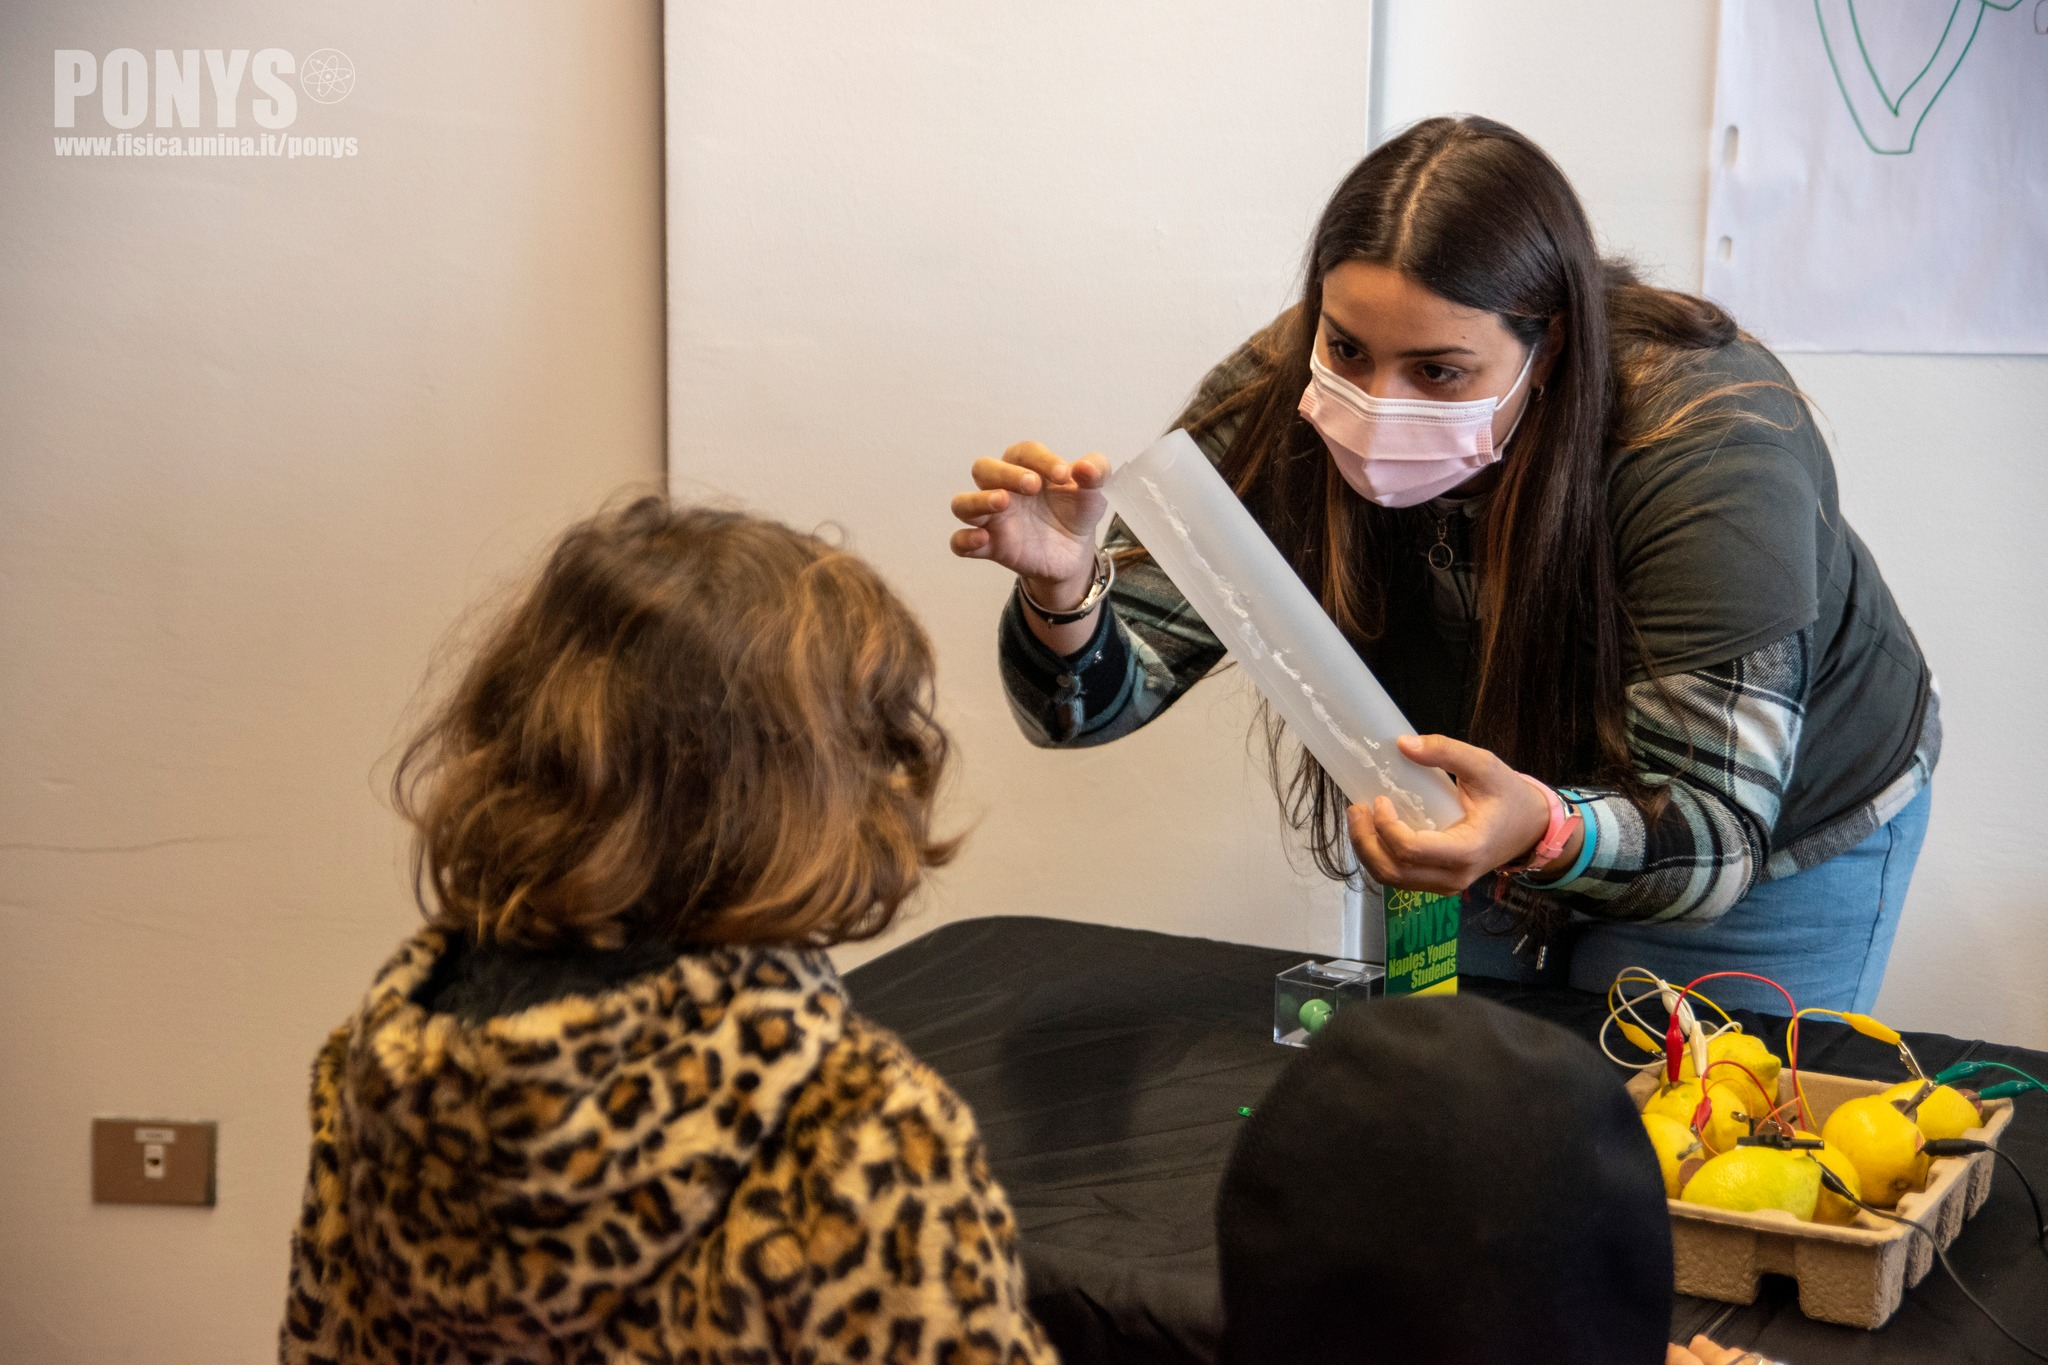
\includegraphics[width=\linewidth]{figures/tubo}
  \caption{\label{fig:tubo} Caduta delle biglie dal punto con potenziale
    maggiore a quello con potenziale minore}
\end{figure}


\section{Elettroscopio a foglie}%
\label{sec:elettroscopio}

Concetti: carica elettrica.

L'elettroscopio a foglie è stato ideato dal fisico inglese Abraham Bennet nel
1786 e successivamente perfezionato da Alessandro Volta con il nome di
\emph{elettrometro}.

Nella sua versione più semplice, il dispositivo è costituito da un'asta
verticale metallica che presenta all'estremità inferiore una sottilissima foglia
(d'oro o di stagnola) e in quella superiore un piattello. Un contenitore con
pareti di vetro racchiude la parte inferiore dell'asta e la fogliolina, evitando
che correnti d'aria alterino il movimento della fogliolina stessa.

Lo strumento serve a rivelare la presenza di cariche elettriche su un corpo,
fornendo anche valutazioni quantitative. Se il piattello superiore non è carico,
la foglia, per gravità, si dispone verticalmente. Se invece esso viene toccato
con un corpo conduttore carico, una parte di questa carica si distribuisce sul
conduttore. Di conseguenza, la foglia e la parte terminale dell'asta si caricano
dello stesso segno e si respingono: la foglia forma così un angolo che può
essere misurato mediante la scala graduata. Il fenomeno si basa su una delle
proprietà fondamentali dell'elettrostatica: corpi dotati di carica elettrica
dello stesso segno si respingono, mentre quelli di segno opposto si attraggono.

Come costruirlo\footnote{
  \url{https://faidatemania.pianetadonna.it/come-costruire-un-elettroscopio-52822.html}
}. Video\footnote{ \url{https://www.youtube.com/watch?v=V2h59o8fKlE} }.

\subsection{Materiale}%
\label{subsec:elettroscopio-materiale}

\begin{itemize}
  \item Senza scala graduata\footnote{
        \url{https://www.mlsystems.it/prodotto/elettroscopio-a-foglia/} }
        (preferibile): 12,50€
  \item Con scala graduata\footnote{
        \url{https://www.mlsystems.it/prodotto/elettroscopio-a-foglie/} }:
        29,50€
  \item Molti barattoli di vetro (riciclati)
  \item Chiodi o viti
  \item Carta stagnola
\end{itemize}

Prezzo totale: 12,50 + 2 + 8 = 22,50€ oppure 29,50 + 2 + 8 = 39,50€.

\section{Elettricità dai limoni}%
\label{sec:limoni}

Costruiamo una batteria con dei limoni!\footnote{
  \url{https://www.scientificamerican.com/article/generate-electricity-with-a-lemon-battery}
} Gli acidi contenuti nei limoni e in tanti frutti e ortaggi hanno la capacità
di generare una differenza di potenziale sotto le giuste condizioni. Si usano
monete da 5 centesimi (rame) e rondelle (zinco) come elettrodi della pila. Ogni
limone può generare una differenza di potenziale attorno ai 0,6V. Per alimentare
un LED si possono usare 6 o più limoni messi in serie, collegando l'anodo di uno
col catodo dell'altro. In base alla durata prevista dell'attività, tenere più
limoni di scorta, perché quelli in uso potrebbero scaricarsi nel corso della
giornata.

\begin{figure}[ht]
  \centering
  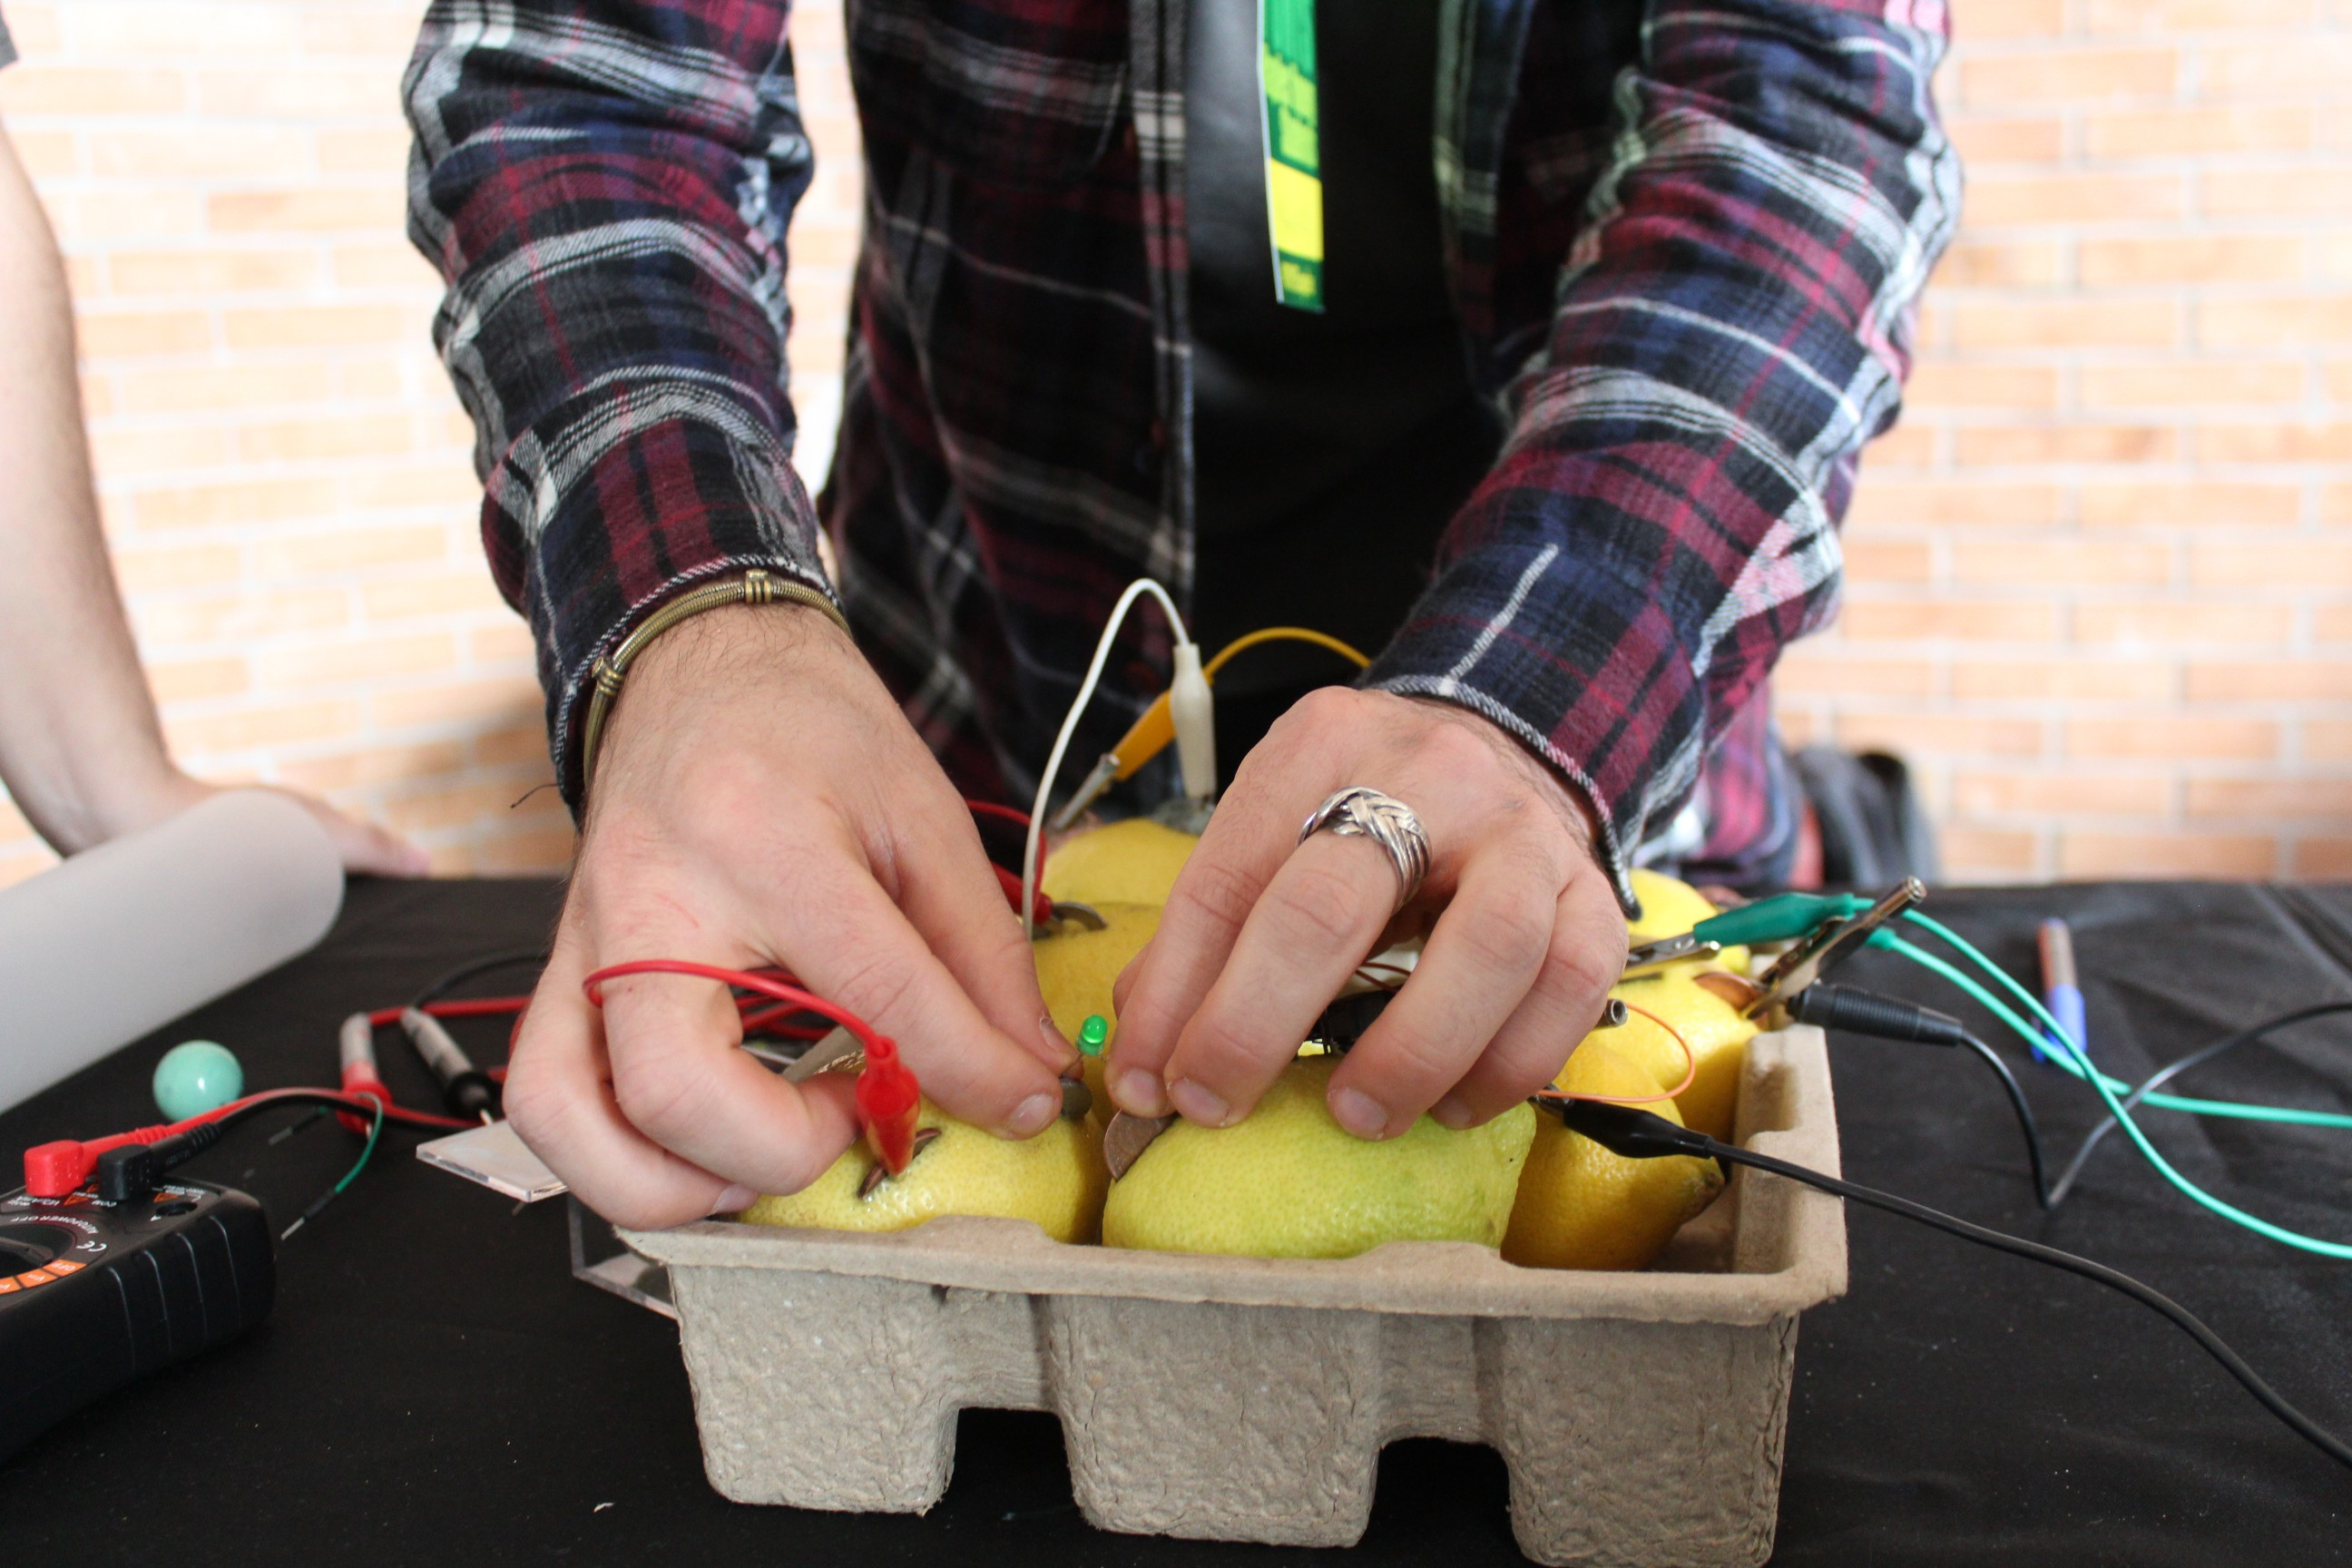
\includegraphics[width=\linewidth]{figures/limoni}
  \caption{\label{fig:limoni} LED che si accende con una pila di limoni}
\end{figure}

\section{Basi dei circuiti}%
\label{sec:inchiostro}

Con una penna a inchiostro conduttivo si spiega il funzionamento base di un
circuito elettrico, in particolare della pila appena realizzata con i limoni. Si
spiega come un circuito debba essere chiuso affinché possa scorrere la corrente.
Su un foglio di carta (può andare bene un A3) si fa disegnare un circuito a
proprio piacimento, che colleghi una differenza di potenziale a un carico. Si
può usare la batteria a limone, una batteria convenzionale, un generatore di
tensione. Come carico può andare bene un LED rosso. Si può consultare il
preventivo sulle note online per il materiale da acquistare\footnote{
  \url{https://www.notion.so/Circuito-con-inchiostro-conduttivo-c7de010dc093499c97812943a7028195}
}.

Perché l'inchiostro conduca è conveniente che il tratto sia abbondante. Questo
significa che ci vuole un po' di tempo per asciugarsi e va preparato prima
facendo più passate.

Risulta abbastanza semplice produrre in casa una pittura conduttiva\footnote{
  \url{https://www.bareconductive.com/blogs/resources/how-to-make-conductive-paint}
}.

In passato si usava la pasta di sale. Si preparavano due paste di colori
diversi, per contraddistinguerle. Una era fatta con molto sale, l'altra usando
invece lo zucchero. Si osservava che una era conduttiva e una isolante, quando
le si usavano per creare circuiti di plastilina in cui infilzare gli elementi
circuitali. Si può pensare di usare anche della carta argentata, tagliata a
striscioline e stesa sulla carta, oppure accartocciata come grossi fili.

\section{Makey Makey}%
\label{sec:makeymakey}

Concetti: circuito elettrico, resistenza, induttanza, messa a terra, messa a
massa.

Manuale ufficiale\footnote{
  \url{https://cdn.shopify.com/s/files/1/0162/8612/files/Makey_Makey_Educators_Guide.pdf?16481577170705338427}
}.

Makey Makey combina realtà fisica e internet, permettendo di usare oggetti di
uso comune per controllare circuiti e computer. Crea un touchpad con qualsiasi
materiale conduttore attaccandolo a Makey Makey tramite le pinze a coccodrillo.

Cosa posso fare con Makey Makey? Dipende da te! Carica un programma a un
computer o un qualsiasi sito web (sì, navigare in internet è il primo step per
ispirarsi e inventare!) e lascia libera l'immaginazione. Diciamo che ti viene
voglia di creare un piano. Ora, anziché usare la solita noiosa tastiera del
computer perché non crei qualcosa di divertente, ad esempio collegando delle
banane al tuo kit Makey Makey, in modo che le banane stesse diventino i tasti
del tuo pazzo piano! Oppure gioca a Pacman utilizzando una comune matita come
joystick! Hai un'idea migliore? Facci sapere cosa farai con il tuo kit Makey
Makey!

Video dimostrativo\footnote{ \url{https://www.youtube.com/watch?v=Ia7r7y_3BIM}
}.

\subsection{Esperimento}%
\label{subsec:makeymakey-esperimento}

Ogni tasto della board sarà collegato a un limone (preferibilmente di Sorrento)
mediante fili di rame non rivestito (non quello per gli avvolgimenti delle
bobine). Si crea una postazione dove ogni limone (quindi il pulsante
corrispondente collegato) sarà controllato da un utilizzatore. Il gruppo
collaborerà giocando a un vecchio gioco arcade mediante la scheda. Ogni team
guadagnerà un punteggio e saranno segnati sulla \emph{lavagna dei vincenti}.

\subsection{Materiale}%
\label{subsec:makeymakey-materiale}

\begin{itemize}
  \item Board Makey Makey\footnote{
        \url{https://makeymakey.com/products/makey-makey-kit} }: 49,90€
  \item Limoni (di Sorrento)
  \item Rame
  \item Un computer
  \item Lavagna dei vincenti
\end{itemize}

Prezzo totale: 49,90 + 10,10 = 60€

\section{Fotoresistenza}%
\label{sec:fotoresistenza}

\begin{figure}[ht]
  \centering
  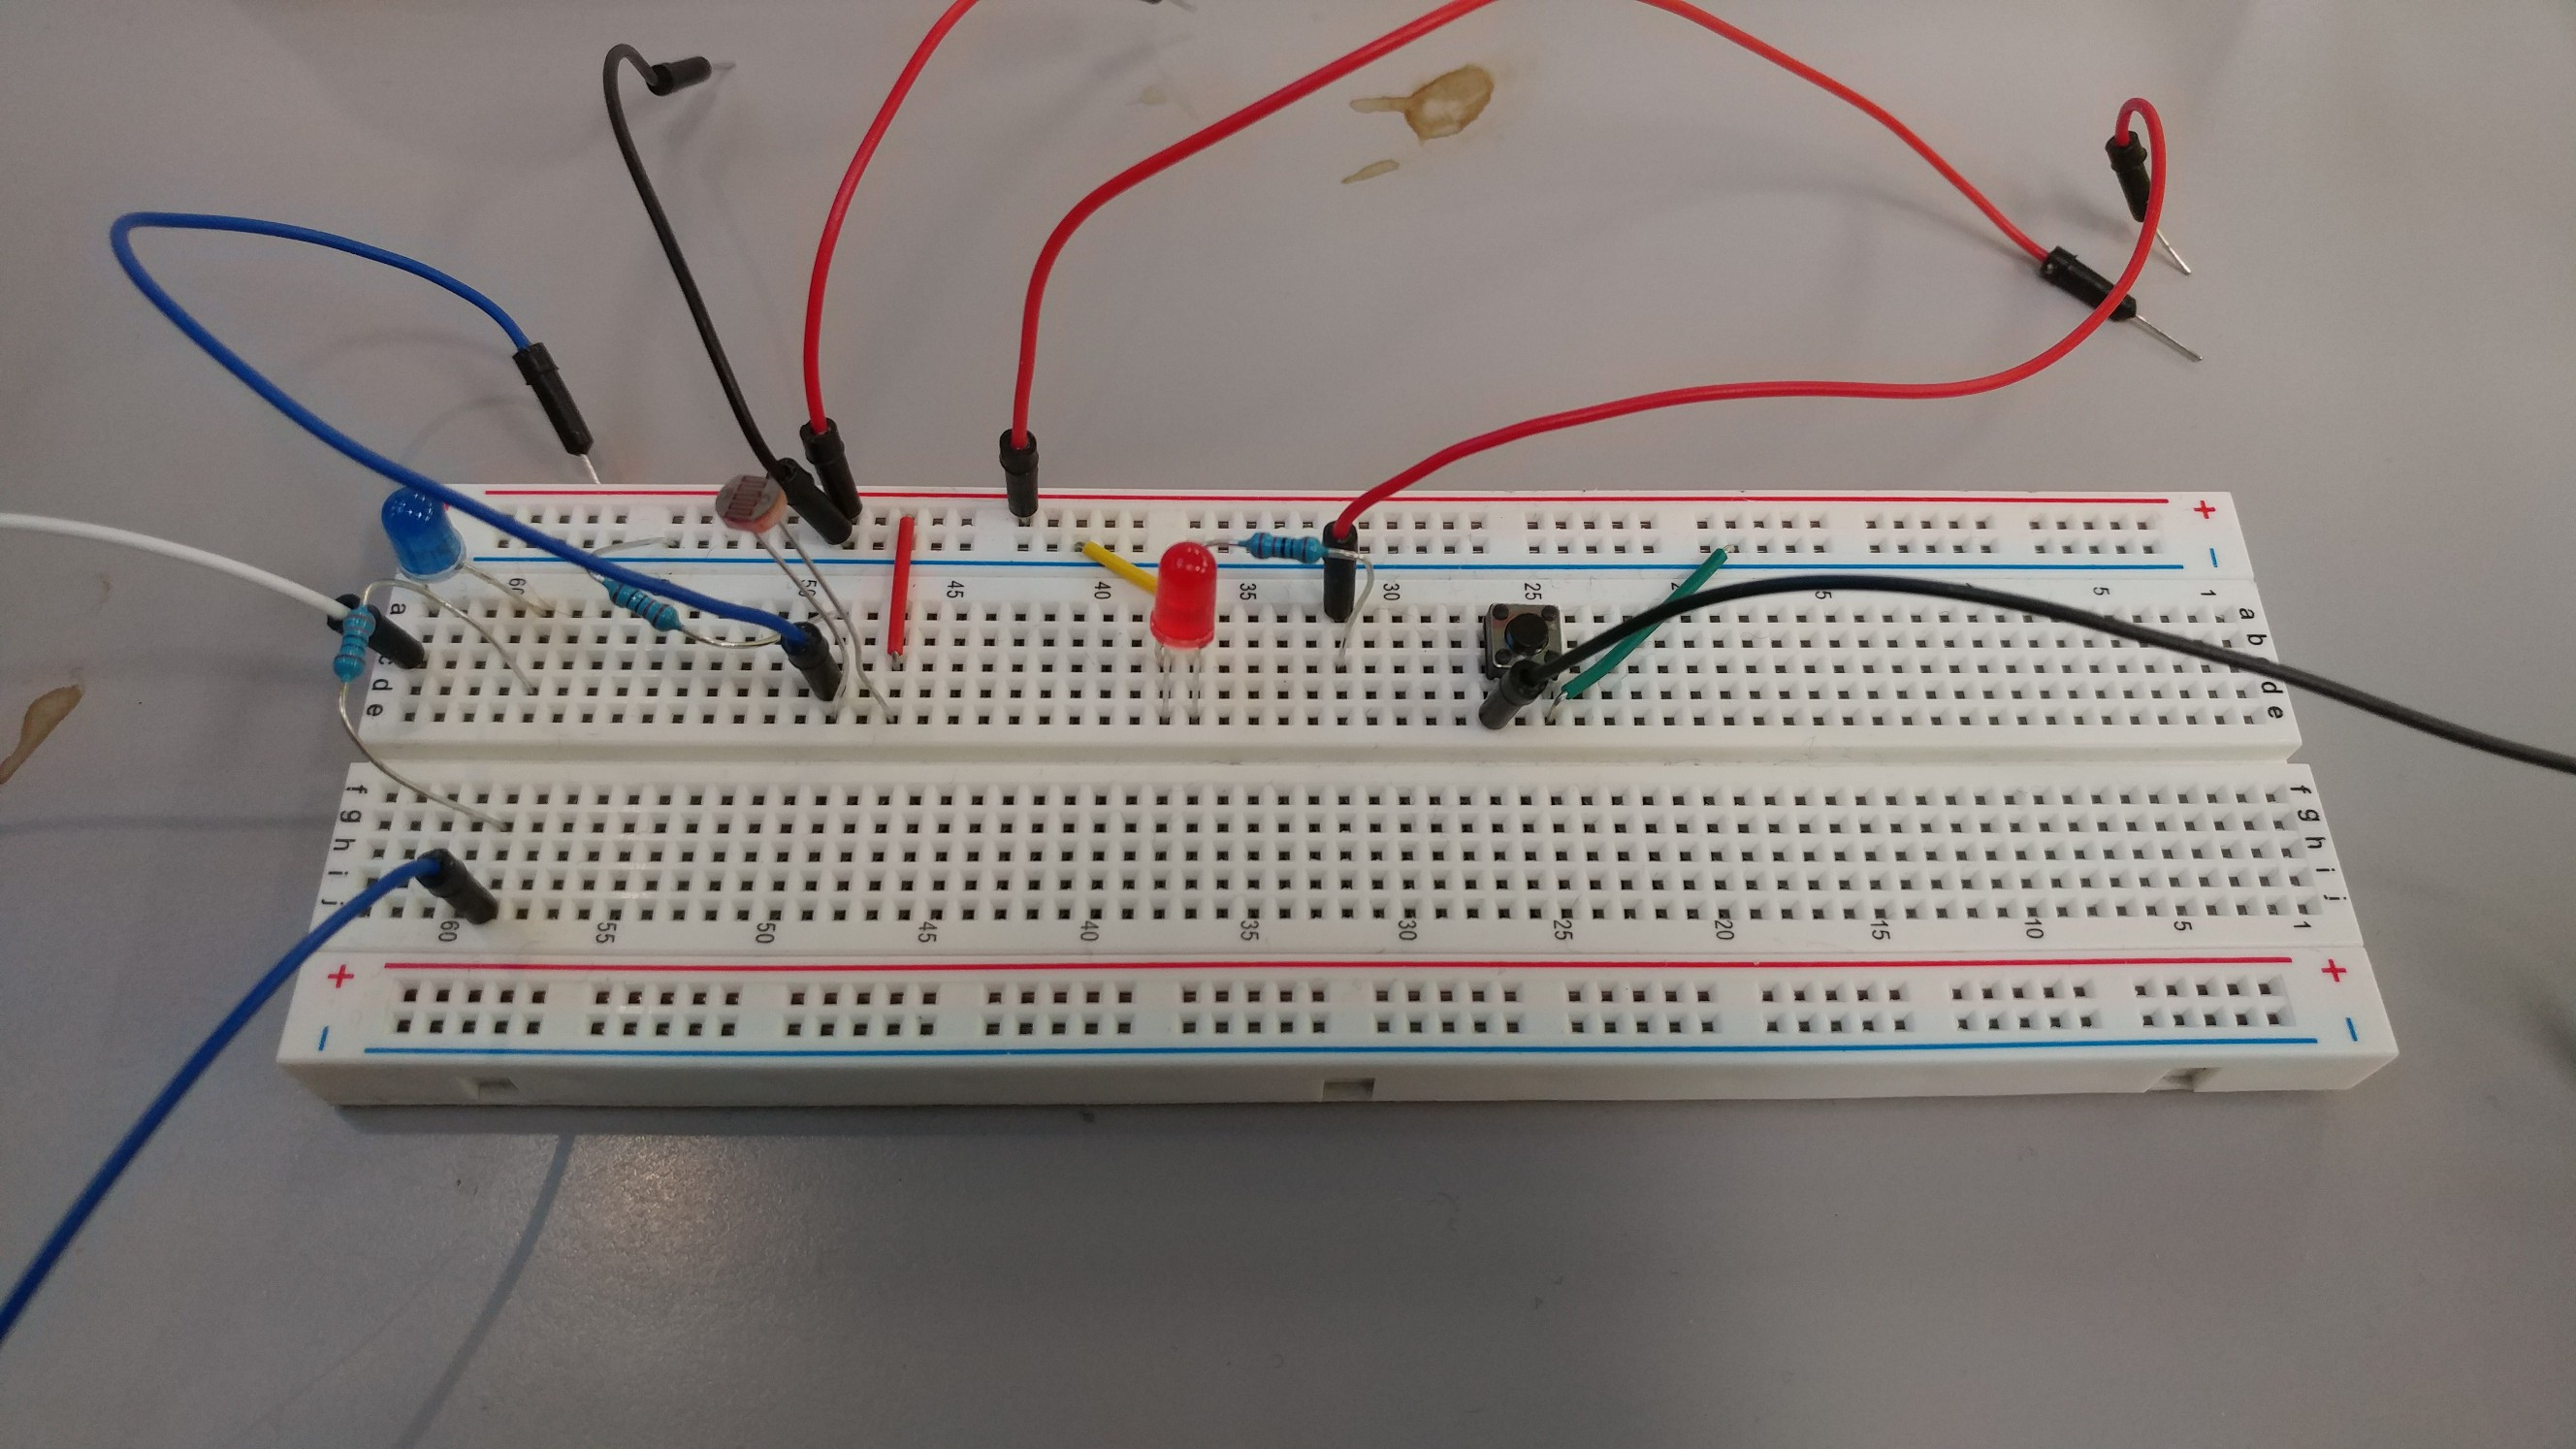
\includegraphics[width=\linewidth]{figures/fotoresistenza}
  \caption{\label{fig:fotoresistenza} Configurazione del circuito con la fotoresistenza}
\end{figure}

Si monta sulla basetta sperimentale il circuito in
figura~\ref{fig:fotoresistenza}, costituito da un sistema di LED, bilanciati con
appropriate resistenze in modo che non si brucino per sovratensione, e di una
foto-resistenza. Illuminando la foto-resistenza si nota che i LED cambiano
comportamento. Questo sistema può essere usato ad esempio per lo sviluppo di
sensori che, in base alla luminosità ambientale, controllino applicazioni di
domotica. Photocells\footnote{
  \url{https://learn.adafruit.com/photocells/arduino-code}}. How to Use a
Photoresistor (or Photocell) --- Arduino Tutorial\footnote{
  \url{https://www.instructables.com/How-to-use-a-photoresistor-or-photocell-Arduino-Tu/}}.

\section{Contatore digitale}%
\label{sec:contatore}

Ci si avvicina all'elettronica digitale descrivendo alcuni dispositivi più
complessi. Si mostra il funzionamento di un contatore con display a 7 segmenti.
Il dispositivo è dotato di un pin per la messa a terra e un pin per la tensione
di alimentazione. Li si riconosce dalle piste stampate più spesse sul retro.
Quattro pin dati trasmettono l'informazione sul numero desiderato, alzando o
abbassando la tensione per ciascun bit corrispondente. Si possono collegare a
degli interruttori oppure collegare direttamente i ponticelli sulla basetta
sperimentale. Si predisponga un foglio con le traduzioni tra binario ed
esadecimale e si chieda agli spettatori di produrre un numero a scelta vostra o
loro.

\begin{figure}[ht]
  \centering
  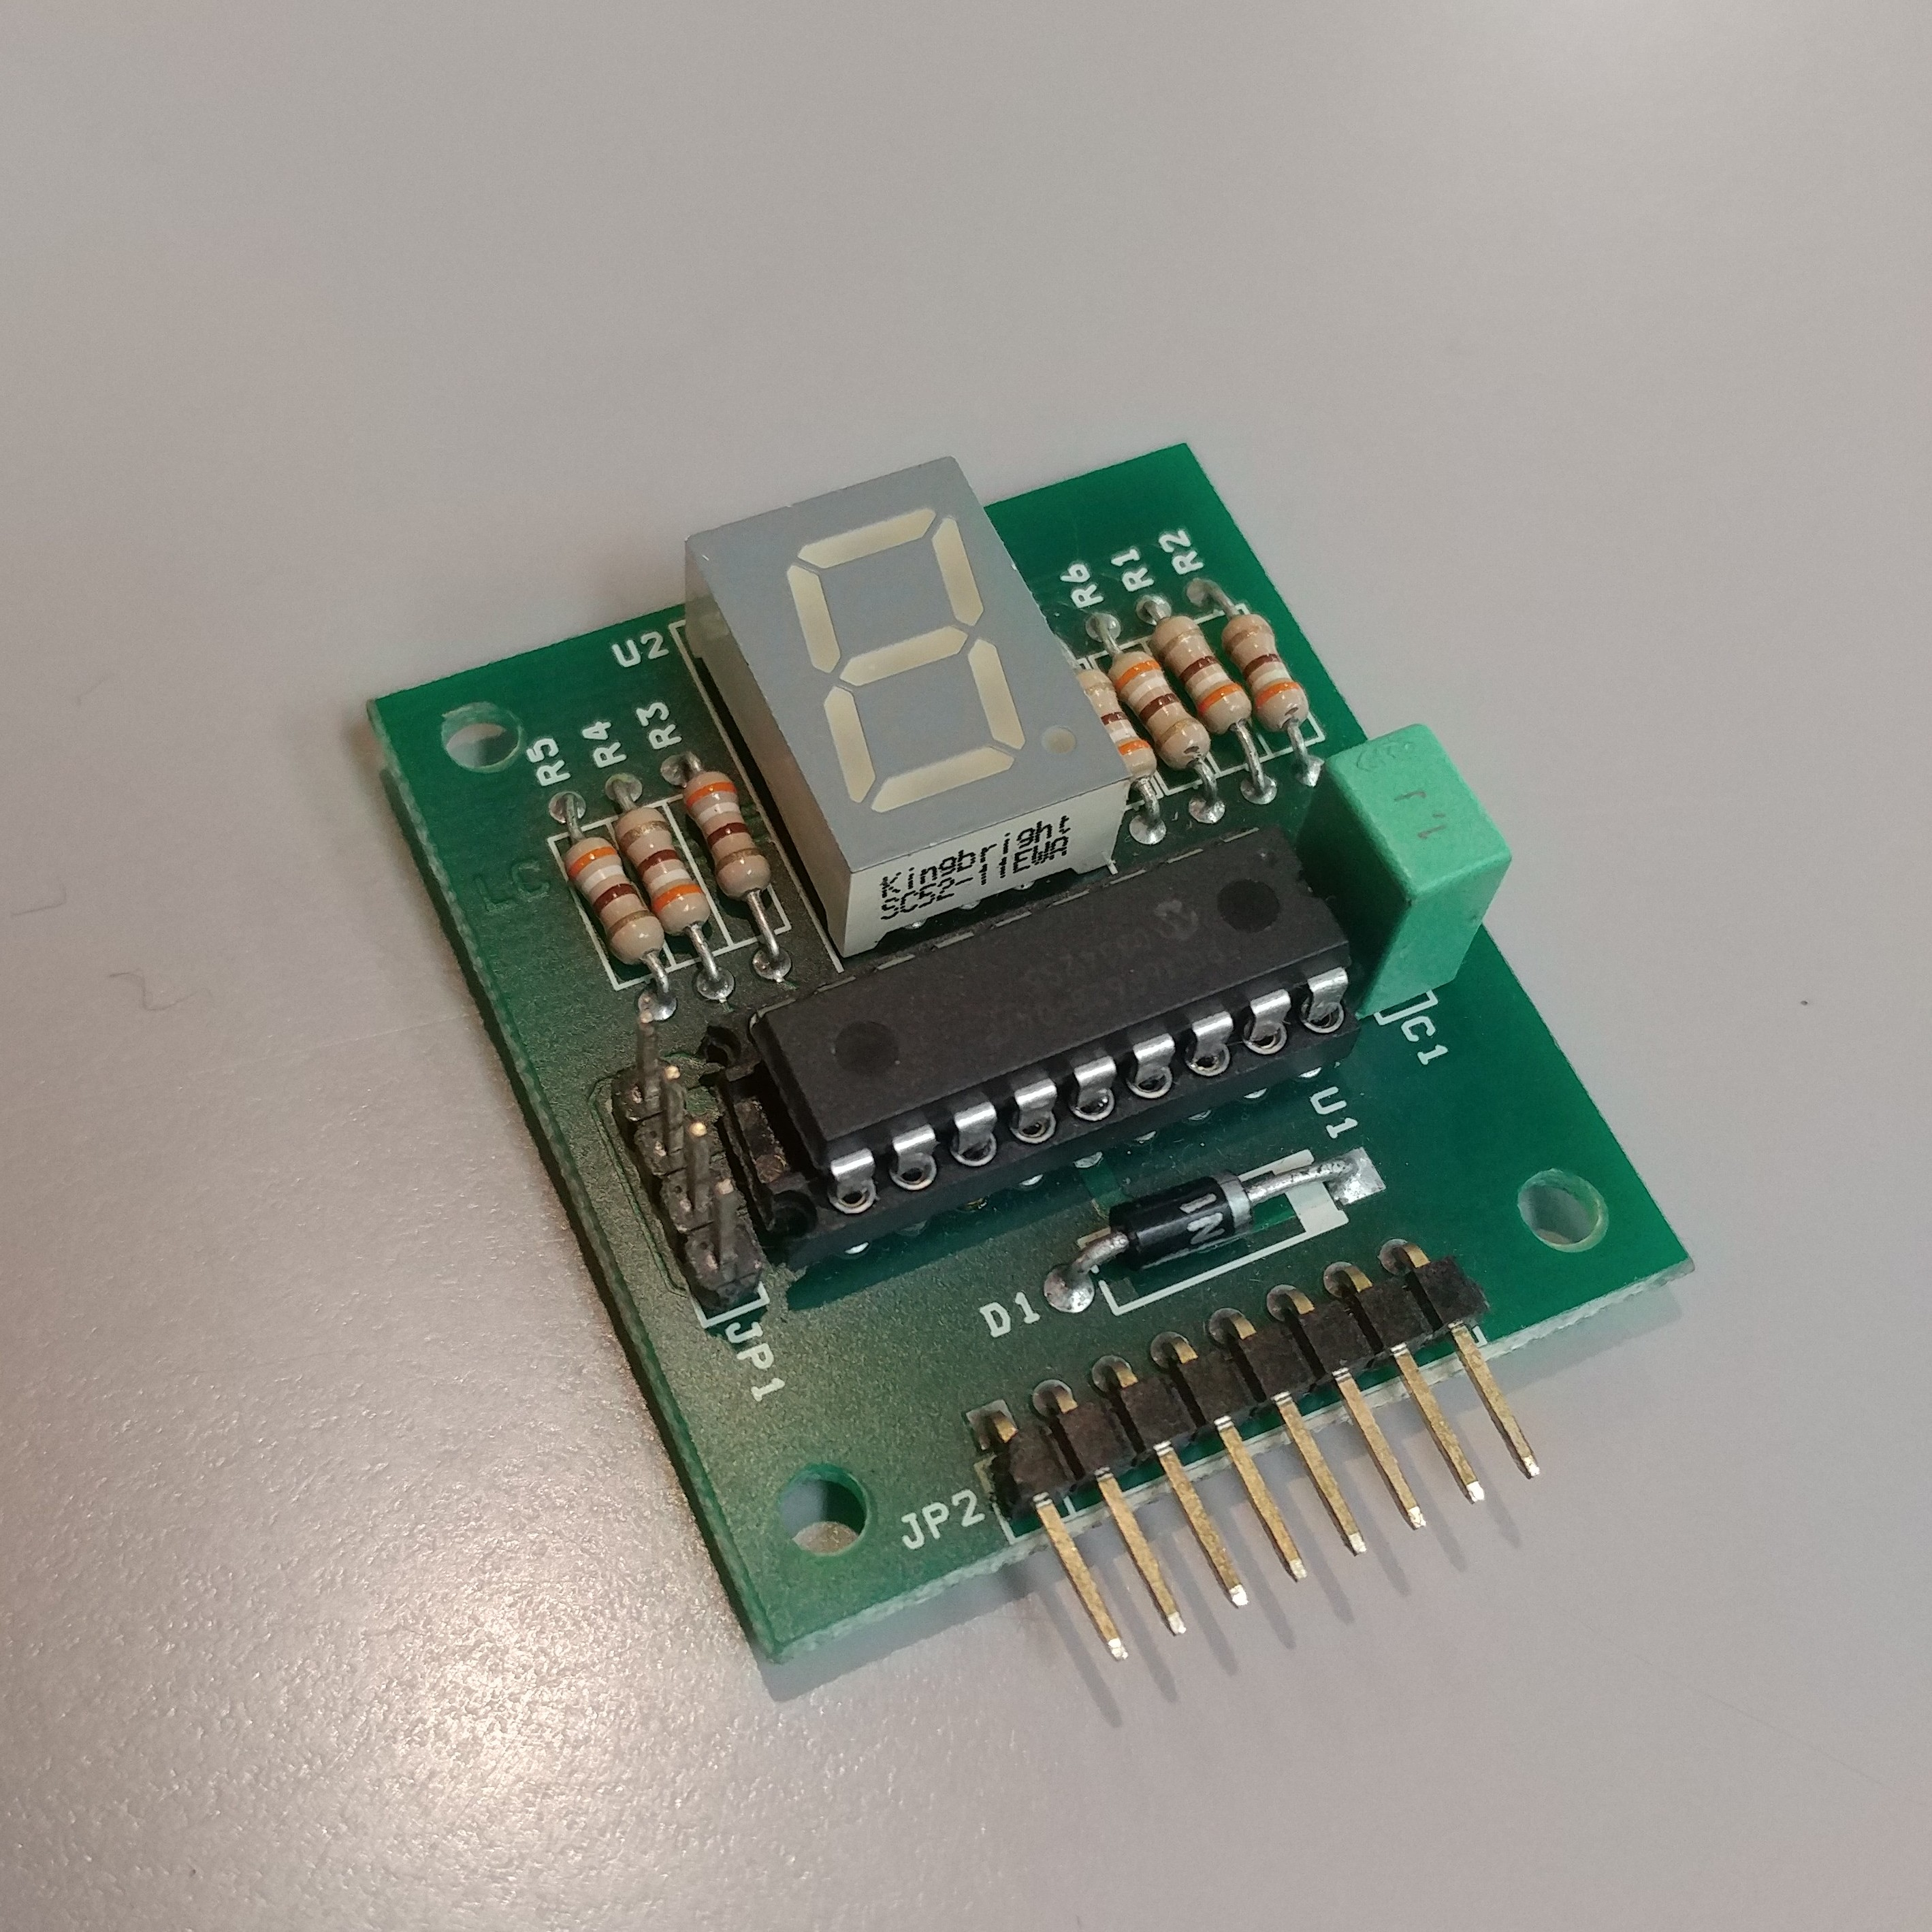
\includegraphics[width=\linewidth]{figures/contatore}
  \caption{\label{fig:contatore} Contatore usato nel corso di lab. 3}
\end{figure}

\begin{figure}[ht]
  \centering
  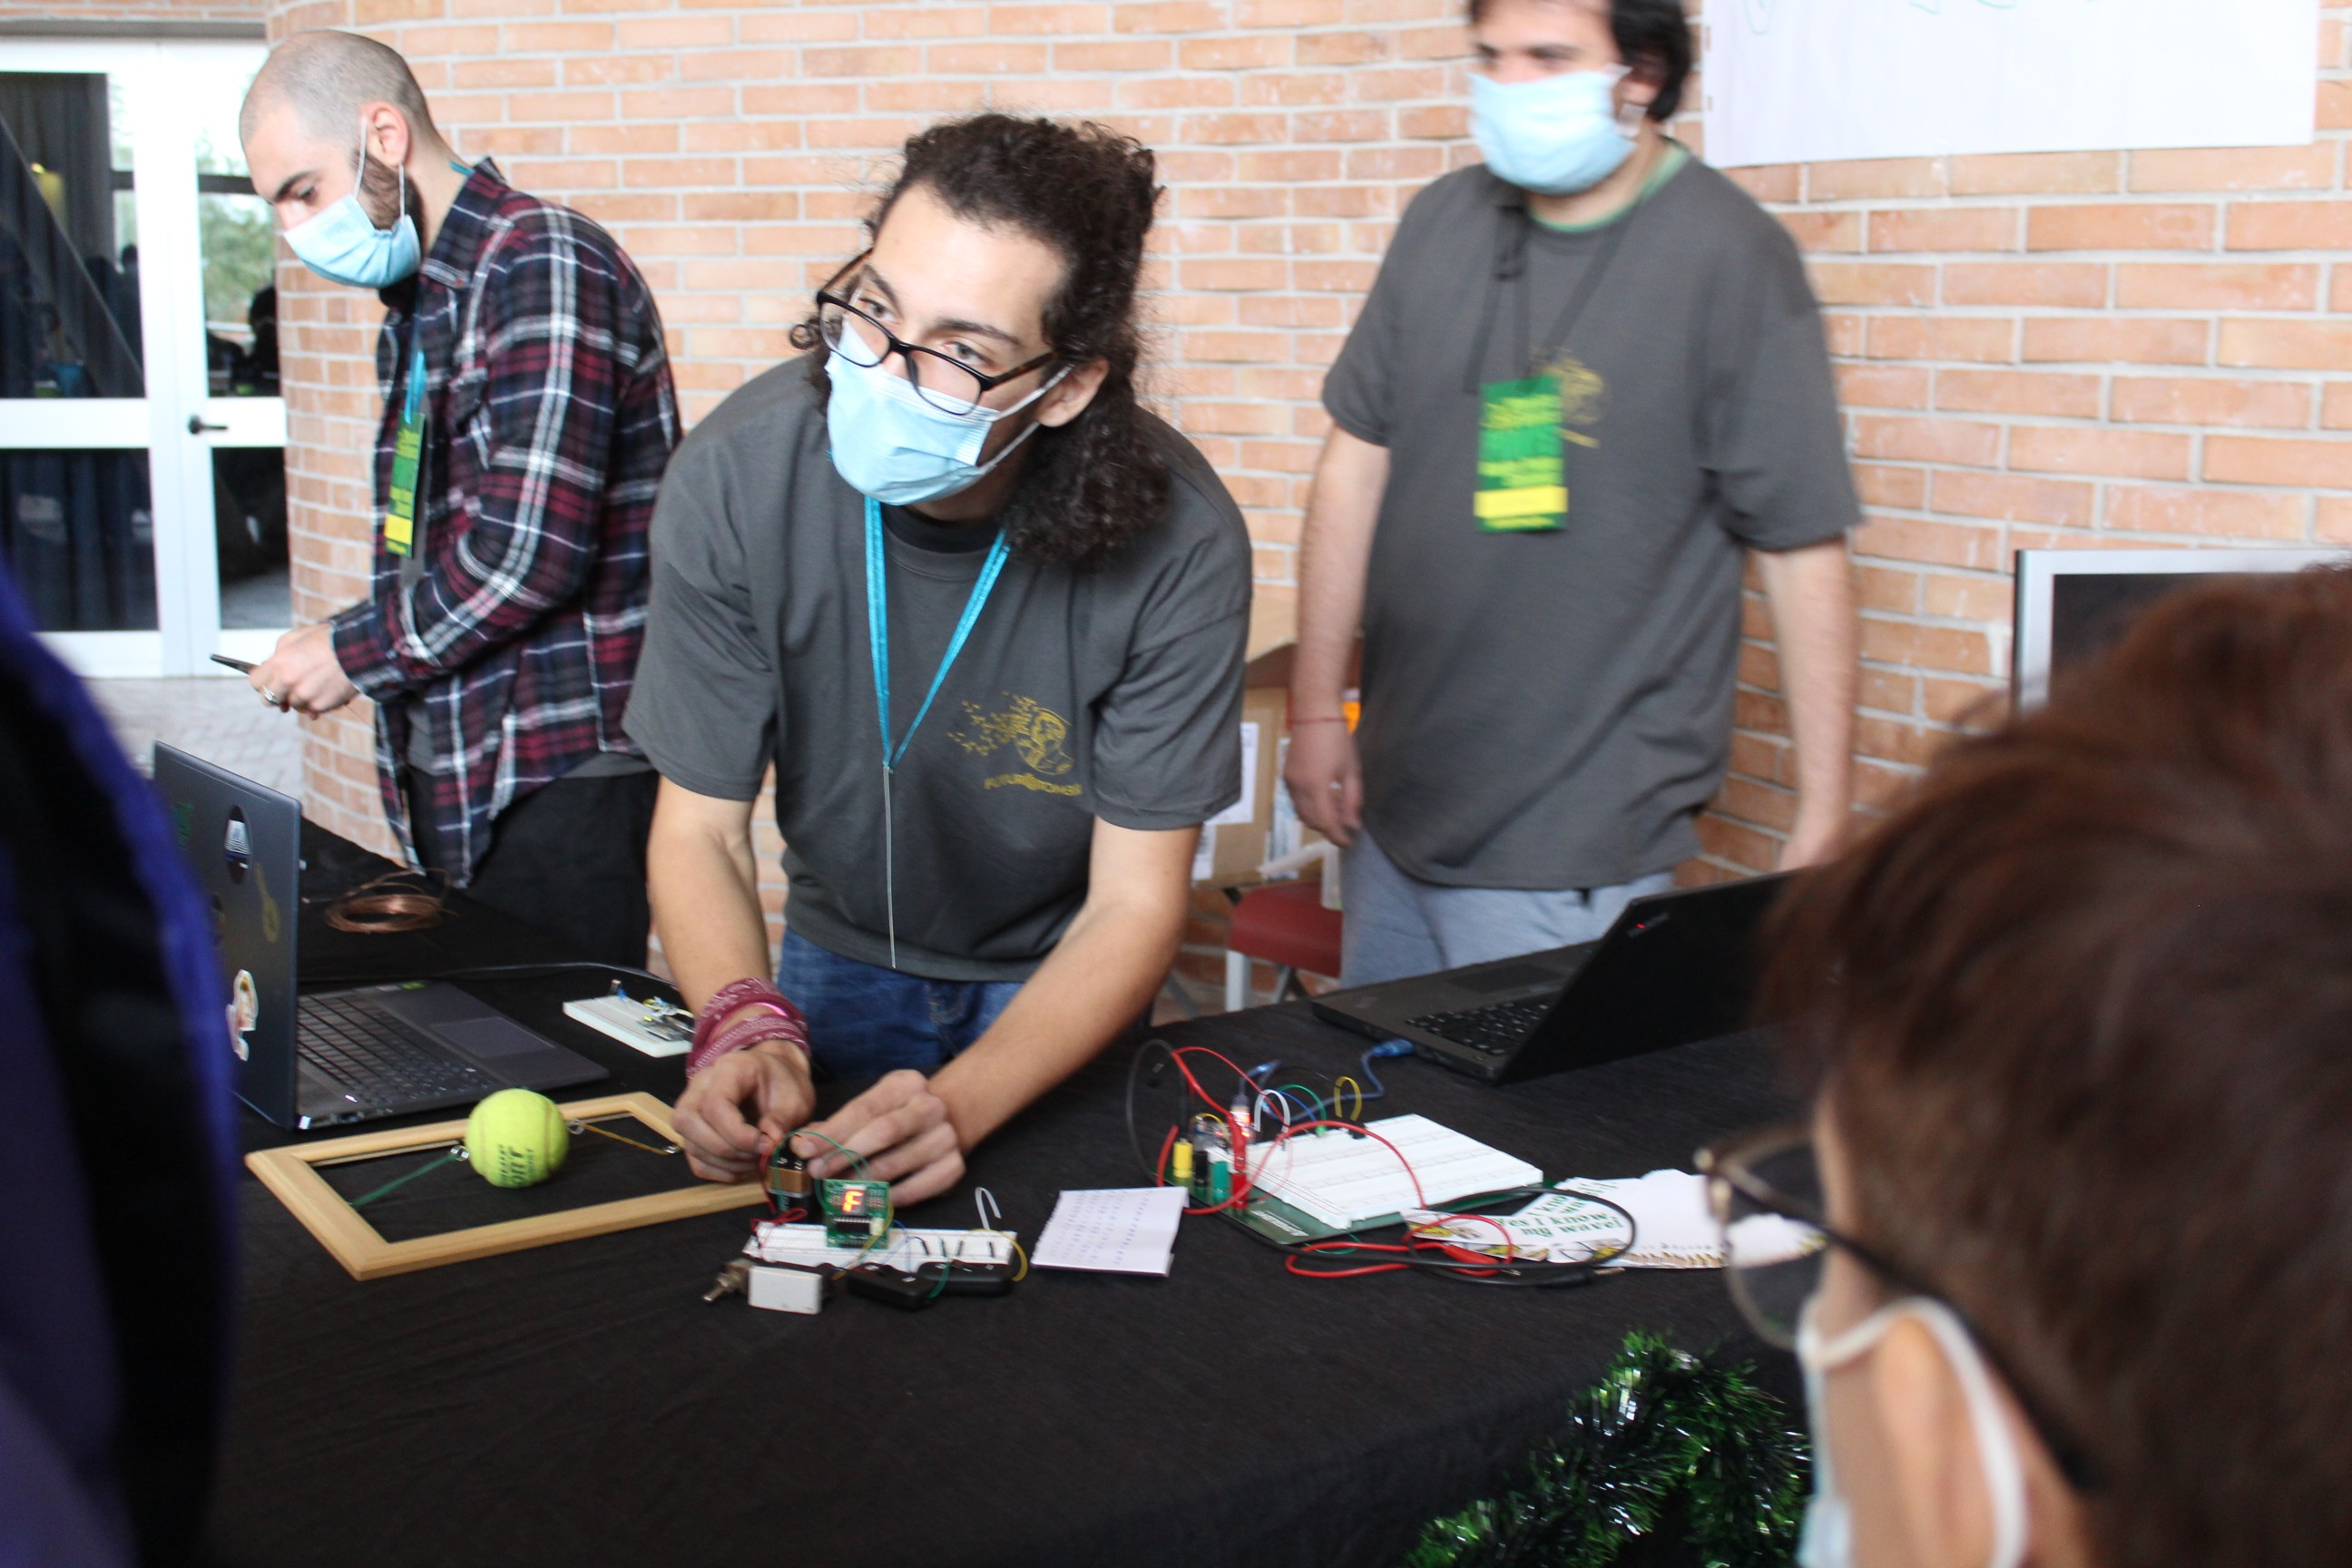
\includegraphics[width=\linewidth]{figures/banchetto_contatore}
  \caption{\label{fig:contatore-banchetto} Banchetto con il contatore montato}
\end{figure}


\section{Luci e musica con Arduino}%
\label{sec:arduino}

Concetti: microcontrollore, programmazione, \emph{open source}.

Arduino è una piattaforma hardware composta da una serie di schede elettroniche
dotate di un microcontrollore. Con Arduino si possono realizzare in maniera
relativamente rapida e semplice piccoli dispositivi come cotrollori di luci, di
velocità per motori, sensori di luce, automatismi per il controllo della
temperatura e dell'umidità e molti altri progetti che utilizzano sensori,
attuatori e la comunicazione con altri dispositivi. La scheda è abbinata a un
semplice ambiente di sviluppo integrato per la programmazione del
microcontrollore. Tutto il software a corredo è libero e gli schemi circuitali
sono distribuiti come hardware libero; per questo motivo è molto utilizzato
nella didattica. La piattaforma fisica si basa su un circuito stampato che
integra un microcontrollore con dei pin connessi alle porte I/O, un regolatore
di tensione e, quando necessario, un'interfaccia USB che permette la
comunicazione con il computer utilizzato per programmare. A questo hardware
viene affiancato un ambiente di sviluppo integrato (IDE) multipiattaforma
disponibile per Linux, Mac e Windows. Questo software permette anche ai novizi
di lavorare con Arduino, in quanto i programmi sono scritti in un linguaggio di
programmazione semplice e intuitivo, chiamato \emph{Wiring}, derivato dal C e
dal C++.

\subsection{Arduino IDE}%
\label{subsec:arduino_ide}

L'ambiente di sviluppo integrato (IDE) di Arduino è un'applicazione
multipiattaforma in Java, derivata dall'IDE creato per il linguaggio di
programmazione Processing e per il progetto Wiring. È possibile scaricare il
software sui canali ufficiali del progetto\footnote{
  \url{https://www.arduino.cc/en/software} }.

\subsection{Esempi di progetto}%
\label{subsec:arduino_esempi}

Con Arduino si possono animare alcuni LED, oppure eseguire una canzoncina con un
altoparlante\footnote{ \url{https://github.com/robsoncouto/arduino-songs.git} }.
Si usano delle resistenze per regolare il volume: messe in serie per diminuirlo,
in parallelo per aumentarlo. Poi si usa un potenziometro come resistenza
variabile per regolare più facilmente il volume. I programmi saranno presi già
fatti e non è necessario un livello elevato di programmazione.

Ogni operatore (volontaria di buona volontà) collaborerà con un ristretto gruppo
di ragazzi (3÷5 giovani spettatori) al fine di utilizzare un Arduino mediante un
pc. La scheda verrà programmata per essere utilizzata come ``stereo'' o per
programmare l'accensione di un LED o come cronometro/orologio. L'obiettivo
formativo è quello di mostrare la versatilità delle singleboard.

\subsection{Materiale}%
\label{subsec:arduino-materiale}

\begin{itemize}
  \item Arduino pezzotto\footnote{ \url{https://www.ebay.it/itm/331535576930} }%
        \textsuperscript{,}\footnote{
        \url{https://www.amazon.it/Elegoo-ATmega328P-ATMEGA16U2-Compatibile-Microcontrollore/dp/B01MRJR8UF}
        }: 12÷16€
  \item Kit completo Arduino pezzotto\footnote{
        \url{https://www.amazon.it/Elegoo-Progetto-Advanced-Principianti-Apprendimento/dp/B01N921CM2}
        }: 44,99€
\end{itemize}

Servirebbero almeno due schede per gestire un traffico di più spettatori. Prezzo
totale: 17,99 + 49,99 = 62,89€

\section{LED nel sughero}%
\label{sec:sughero}

Concetti: diodi, capacità, circuito elettrico di base.

Si realizza un circuito composto da LED e pila a bottone messa dentro un tappo
di sughero, qua tutti abbiamo fatto lab 2 con \emph{Pasqualino Maddalena}. Come
costruirlo\footnote{ \url{https://www.youtube.com/watch?v=dmPNsWBHK8A} }. Il
prodotto realizzato resta agli spettatori.

\subsection{Materiale}%
\label{subsec:sughero-materiale}

\begin{itemize}
  \item 100 tappi di sughero\footnote{
        \url{https://www.amazon.it/decorare-personalizzare-bricolage-bottiglie-accessori/dp/B072VZRWW9}
        } (forse sono troppi): 14,99€
  \item 500 LED\footnote{
        \url{https://www.amazon.it/AUKENIEN-Rotonda-Luminosit\%C3\%A0-Diffusione-Luminosa/dp/B0972D2BMH}
        } (sono decisamente troppi): 9,99€
  \item Due pacchi di 40 pile a bottone da 3,3V\footnote{
        \url{https://www.amazon.it/Confezione-batteria-alcalina-bottone-batterie/dp/B07C1N42W1}
        }: 13,94€
\end{itemize}

Prezzo totale: 2*6,97 + 14,99 + 9,99 = 38,92€

\section{Chiosco arcade}%
\label{sec:arcade}

Questa parte del banchetto è puramente dimostrativa e non prevede spiegazioni
tecniche. Con un Raspberry Pi 0 mettere su una postazione con giochi retro open
source. Si può aggiungere interazione con potenziometri, pulsanti, e così via.
Vedi Freedoom\footnote{ \url{https://freedoom.github.io/} }.
\url{https://www.youtube.com/watch?v=qOUP_0eMDqw}

Materiale da recuperare: schermo, Raspberry Pi 0, joystick.

\begin{figure}[ht]
  \centering
  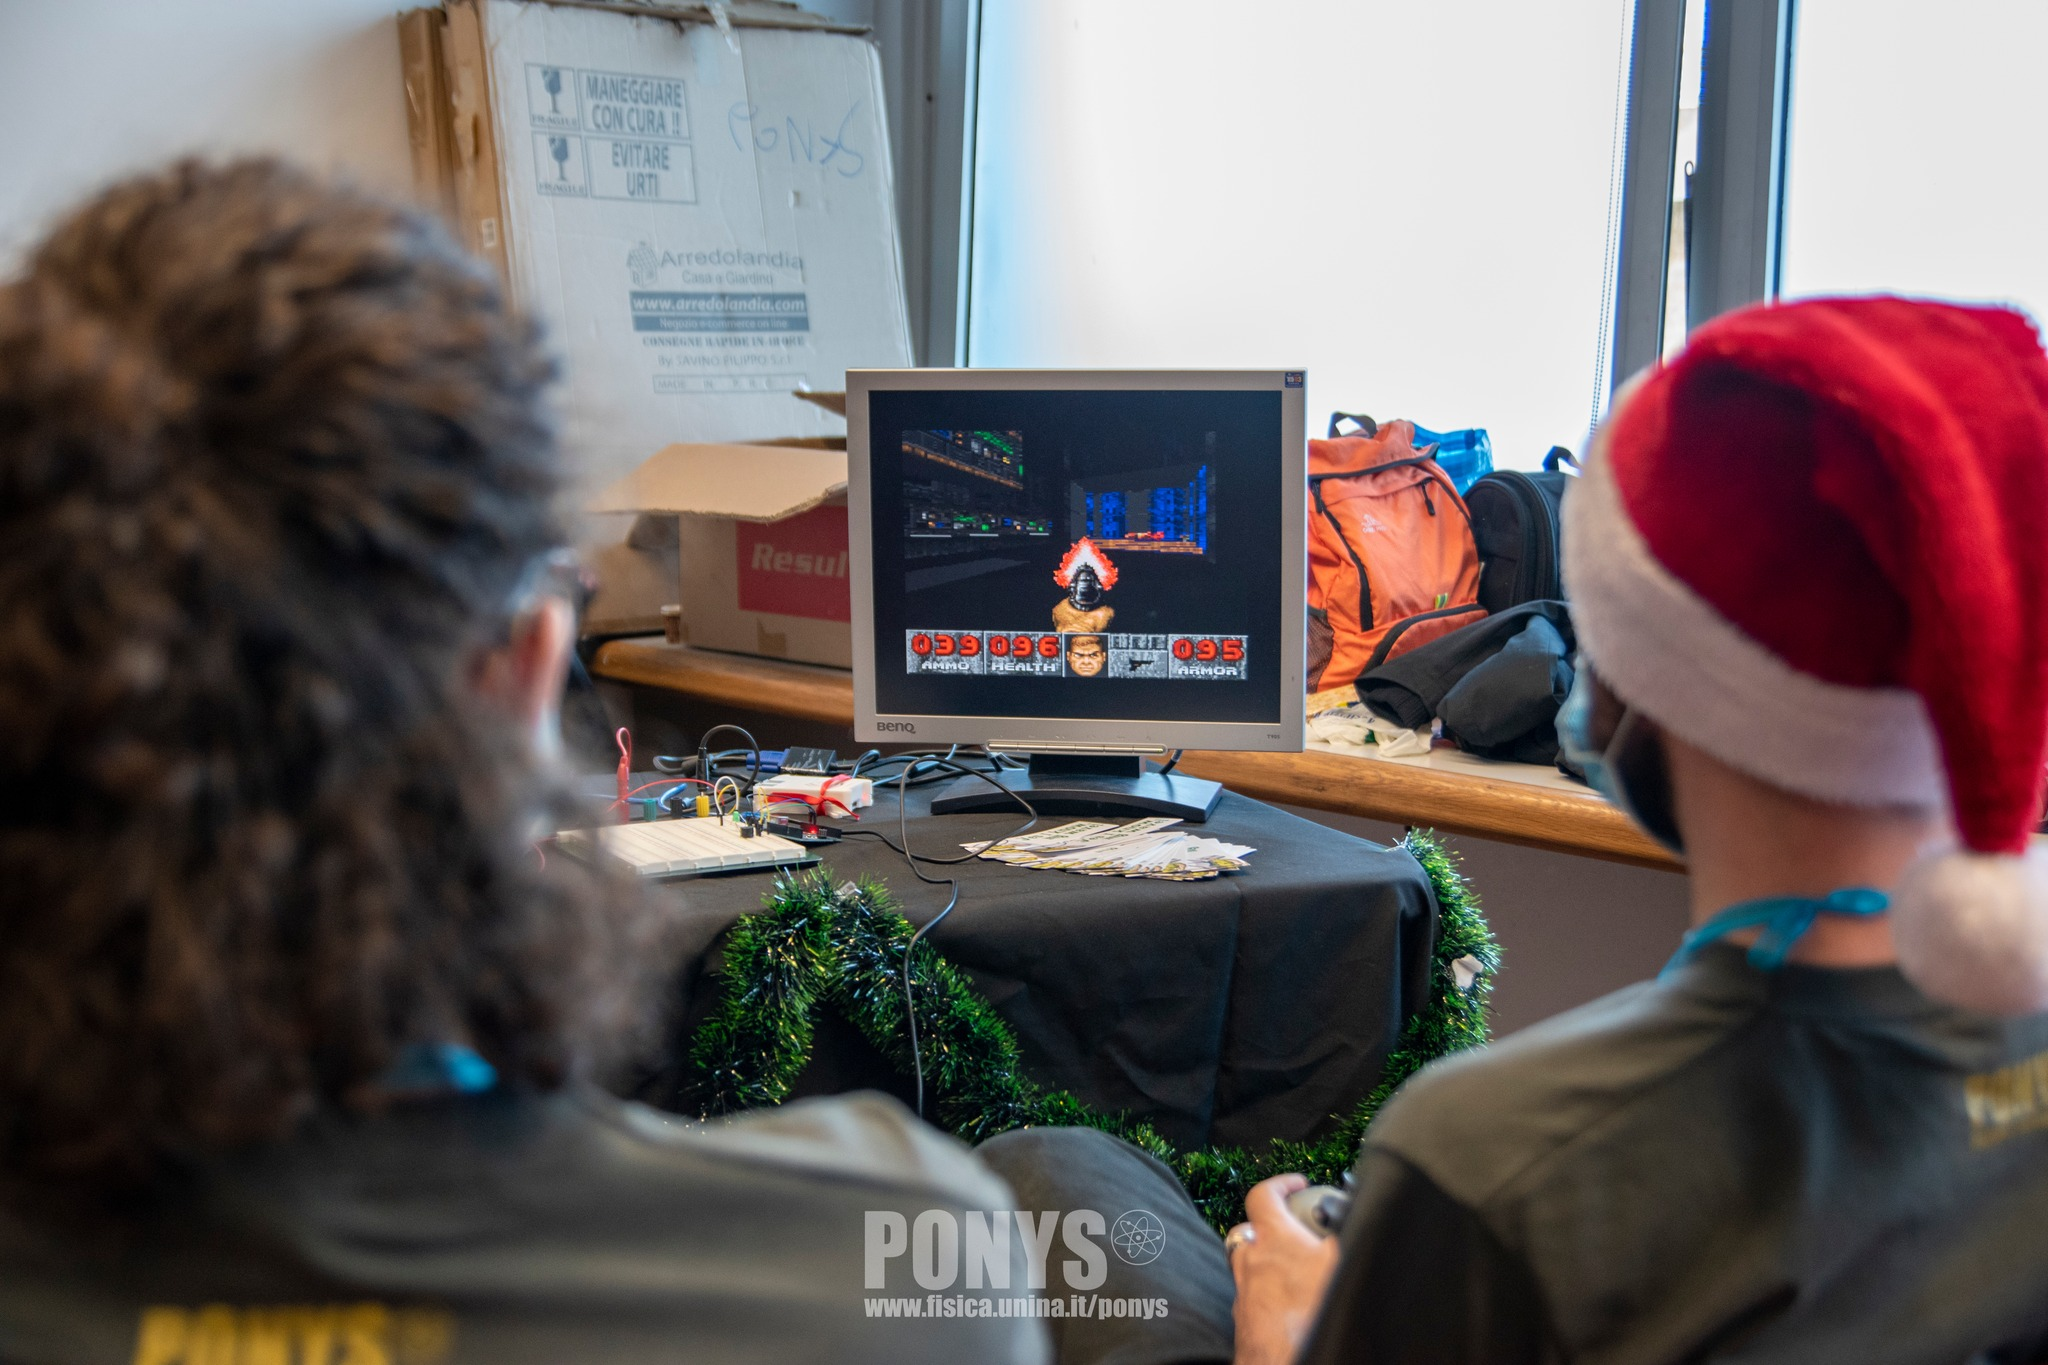
\includegraphics[width=\linewidth]{figures/doom}
  \caption{\label{fig:doom} Videogioco con Doom}
\end{figure}

\section{Sonar o accelerometro}%
\label{sec:sonar-accelerometro}

Si può chiedere a Giancarlo, presso il gruppo di ricerca in didattica con
Balzano, di usare la scheda su cui è montato un accelerometro. I dati misurati
da questo sono trasmessi tramite Wi-Fi ai dispositivi che si connettono e si
possono osservare le componenti dell'accelerazione lungo i tre assi cartesiani.

Bisogna chiedere a Giancarlo di rivedere questi esperimenti, che furono portati
all'ultima edizione di Futuro Remoto. Potrebbero esserci alcune componenti da
riacquistare. Far vedere l'app per smartphone Phyphox\footnote{
  \url{https://phyphox.org/} }. Con la molla si spiega il funzionamento
dell'accelerometro.

\section{Extra}%
\label{sec:extra}

Trova più foto sulla pagina Facebook dei PONYS\footnote{
  \url{https://www.facebook.com/ponys.unina/photos/a.1549835678662683/2895353720777532}
}.

\end{document}
